\section{\src{dyn_diffusion}}\label{s:dyn_diffusion}

\subsection{Description}

Kernel \src{dyn_diffusion} is taken from the original subroutine
\src{OPRT_diffusion} in \NICAM.
%
This subroutine is originally defined, as you can see in that name, in module
\src{mod_oprt}.
%
This module defines several differential operators on the sphere, such
as divergence, gradient, etc.
%
Subroutine \src{OPRT_diffusion} calculates diffusion term
 of given scalar field.

\subsection{Discretization and code}


Argument lists and local variables definition part of this subroutine is
as follows.

\begin{LstF90}[name=diffusion,firstnumber=auto]
subroutine OPRT_diffusion( &
     dscl,      dscl_pl,      &
     scl,       scl_pl,       &
     kh,        kh_pl,        &
     coef_intp, coef_intp_pl, &
     coef_diff, coef_diff_pl  )
  implicit none

  real(RP), intent(out) :: dscl        (ADM_gall   ,ADM_kall,ADM_lall   )
  real(RP), intent(out) :: dscl_pl     (ADM_gall_pl,ADM_kall,ADM_lall_pl)
  real(RP), intent(in)  :: scl         (ADM_gall   ,ADM_kall,ADM_lall   )
  real(RP), intent(in)  :: scl_pl      (ADM_gall_pl,ADM_kall,ADM_lall_pl)
  real(RP), intent(in)  :: kh          (ADM_gall   ,ADM_kall,ADM_lall   )
  real(RP), intent(in)  :: kh_pl       (ADM_gall_pl,ADM_kall,ADM_lall_pl)
  real(RP), intent(in)  :: coef_intp   (ADM_gall   ,1:3,        ADM_nxyz,TI:TJ,ADM_lall   )
  real(RP), intent(in)  :: coef_intp_pl(ADM_gall_pl,1:3,        ADM_nxyz,      ADM_lall_pl)
  real(RP), intent(in)  :: coef_diff   (ADM_gall   ,1:6,        ADM_nxyz,      ADM_lall   )
  real(RP), intent(in)  :: coef_diff_pl(            1:ADM_vlink,ADM_nxyz,      ADM_lall_pl)

  real(RP) :: vt   (ADM_gall   ,ADM_nxyz,TI:TJ)
  real(RP) :: vt_pl(ADM_gall_pl,ADM_nxyz)
  real(RP) :: kf   (1:6)

  integer  :: gmin, gmax, iall, gall, kall, lall, nxyz, gminm1

  integer  :: ij
  integer  :: ip1j, ijp1, ip1jp1
  integer  :: im1j, ijm1, im1jm1

  integer  :: g, k, l, d, n, v
  !---------------------------------------------------------------------------
\end{LstF90}
%
Here \src{dscl}, \src{dscl_pl} are calculated diffusion of regular
region and polar region, respectively, from some scalar field \src{scl},
\src{scl_pl} and diffusion coefficient \src{kh}, \src{kh_pl} at the triangular points.
%
Other arguments \src{coef_intp}, \src{coef_intp_pl}, \src{coef_diff},
\src{coef_diff_pl} are various coefficients for finite difference
calculation.
%
These coefficients are calculated in advance in the subroutine
\src{OPRT_diffusion_setup}
also defined in the module (See \autoref{dyn_metrics}).
%
These are supplied as arguments, not module variables, because of the computational optimization.
The values are read from input data before executing this subroutine.

local variables
\src{vt}, \src{vt_pl} are the differentiation of given scalar field at
the gravitational center of triangles.
%
Note that the range of the last dimension is \src{TI:TJ}.
%
See below for details.
%
\src{ADM_nxyz} is \src{parameter} and the value is 3, so this dimension
shows spatial direction (X,Y,Z).


The first part of this subroutine is as follows.

\begin{LstF90}[name=diffusion,firstnumber=last]
  call DEBUG_rapstart('OPRT_diffusion')

  gmin = (ADM_gmin-1)*ADM_gall_1d + ADM_gmin
  gmax = (ADM_gmax-1)*ADM_gall_1d + ADM_gmax
  iall = ADM_gall_1d
  gall = ADM_gall
  kall = ADM_kall
  lall = ADM_lall
  nxyz = ADM_nxyz

  gminm1 = (ADM_gmin-1-1)*ADM_gall_1d + ADM_gmin-1

  !$omp parallel default(none),private(g,k,l,d,ij,ip1j,ip1jp1,ijp1,im1j,ijm1,im1jm1), &
  !$omp shared(ADM_have_sgp,gminm1,gmin,gmax,iall,gall,kall,lall,nxyz,dscl,scl,kh,kf,vt,coef_intp,coef_diff)
  do l = 1, lall
  do k = 1, kall

     do d = 1, nxyz
        !$omp do
        do g = gminm1, gmax
           ij     = g
           ip1j   = g + 1
           ip1jp1 = g + iall + 1
           ijp1   = g + iall

           vt(g,d,TI) = ( ( + 2.0_RP * coef_intp(g,1,d,TI,l) &
                            - 1.0_RP * coef_intp(g,2,d,TI,l) &
                            - 1.0_RP * coef_intp(g,3,d,TI,l) ) * scl(ij    ,k,l) &
                        + ( - 1.0_RP * coef_intp(g,1,d,TI,l) &
                            + 2.0_RP * coef_intp(g,2,d,TI,l) &
                            - 1.0_RP * coef_intp(g,3,d,TI,l) ) * scl(ip1j  ,k,l) &
                        + ( - 1.0_RP * coef_intp(g,1,d,TI,l) &
                            - 1.0_RP * coef_intp(g,2,d,TI,l) &
                            + 2.0_RP * coef_intp(g,3,d,TI,l) ) * scl(ip1jp1,k,l) &
                        ) / 3.0_RP
        enddo
        !$omp end do nowait

        !$omp do
        do g = gminm1, gmax
           ij     = g
           ip1j   = g + 1
           ip1jp1 = g + iall + 1
           ijp1   = g + iall

           vt(g,d,TJ) = ( ( + 2.0_RP * coef_intp(g,1,d,TJ,l) &
                            - 1.0_RP * coef_intp(g,2,d,TJ,l) &
                            - 1.0_RP * coef_intp(g,3,d,TJ,l) ) * scl(ij    ,k,l) &
                        + ( - 1.0_RP * coef_intp(g,1,d,TJ,l) &
                            + 2.0_RP * coef_intp(g,2,d,TJ,l) &
                            - 1.0_RP * coef_intp(g,3,d,TJ,l) ) * scl(ip1jp1,k,l) &
                        + ( - 1.0_RP * coef_intp(g,1,d,TJ,l) &
                            - 1.0_RP * coef_intp(g,2,d,TJ,l) &
                            + 2.0_RP * coef_intp(g,3,d,TJ,l) ) * scl(ijp1  ,k,l) &
                        ) / 3.0_RP
        enddo
        !$omp end do
     enddo

     if ( ADM_have_sgp(l) ) then ! pentagon
        !$omp master
        vt(gminm1,XDIR,TI) = vt(gminm1+1,XDIR,TJ)
        vt(gminm1,YDIR,TI) = vt(gminm1+1,YDIR,TJ)
        vt(gminm1,ZDIR,TI) = vt(gminm1+1,ZDIR,TJ)
        !$omp end master
     endif
\end{LstF90}

In the first part, \src{vt(:,:,TI)}, \src{vt(:,:,TJ)} are calculated
from \src{scl} with interpolation.
\autoref{f:interpolation_for_vt} shows grid arrangements.
\src{scl} are defined on white circle points in the figure,
and \src{vt} are defined on black circle points.
See \autoref{f:interpolation_for_dscl} for grid arrangement.
\src{vt} is defined on the black circle points in the figure,
while other physical quantities are defined on the white circle points.

\begin{figure}[htpb]
 \centering
 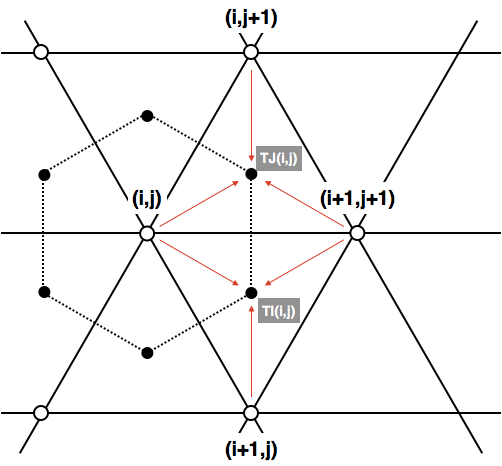
\includegraphics[scale=.4]{figs/diffusion_intp.png}
 \caption{interpolation for \src{vt}}
 \label{f:interpolation_for_vt}
\end{figure}


The second part of this subroutine is as follows.

\begin{LstF90}[name=diffusion,firstnumber=last]
!OCL XFILL
     !$omp do
     do g = 1, gmin-1
        dscl(g,k,l) = 0.0_RP
     enddo
     !$omp end do nowait

     !$omp do
     do g = gmin, gmax
        ij     = g
        ip1j   = g + 1
        ip1jp1 = g + iall + 1
        ijp1   = g + iall
        im1j   = g - 1
        im1jm1 = g - iall - 1
        ijm1   = g - iall

        kf(1) = 0.5_RP * ( kh(ij    ,k,l) + kh(ip1jp1,k,l) )
        kf(2) = 0.5_RP * ( kh(ij    ,k,l) + kh(ijp1  ,k,l) )
        kf(3) = 0.5_RP * ( kh(im1j  ,k,l) + kh(ij    ,k,l) )
        kf(4) = 0.5_RP * ( kh(im1jm1,k,l) + kh(ij    ,k,l) )
        kf(5) = 0.5_RP * ( kh(ijm1  ,k,l) + kh(ij    ,k,l) )
        kf(6) = 0.5_RP * ( kh(ij    ,k,l) + kh(ip1j  ,k,l) )

        dscl(g,k,l) = ( kf(1) * coef_diff(g,1,XDIR,l) * ( vt(ij    ,XDIR,TI) + vt(ij    ,XDIR,TJ) ) &
                      + kf(2) * coef_diff(g,2,XDIR,l) * ( vt(ij    ,XDIR,TJ) + vt(im1j  ,XDIR,TI) ) &
                      + kf(3) * coef_diff(g,3,XDIR,l) * ( vt(im1j  ,XDIR,TI) + vt(im1jm1,XDIR,TJ) ) &
                      + kf(4) * coef_diff(g,4,XDIR,l) * ( vt(im1jm1,XDIR,TJ) + vt(im1jm1,XDIR,TI) ) &
                      + kf(5) * coef_diff(g,5,XDIR,l) * ( vt(im1jm1,XDIR,TI) + vt(ijm1  ,XDIR,TJ) ) &
                      + kf(6) * coef_diff(g,6,XDIR,l) * ( vt(ijm1  ,XDIR,TJ) + vt(ij    ,XDIR,TI) ) )
     enddo
     !$omp end do

     !$omp do
     do g = gmin, gmax
        ij     = g
        ip1j   = g + 1
        ip1jp1 = g + iall + 1
        ijp1   = g + iall
        im1j   = g - 1
        im1jm1 = g - iall - 1
        ijm1   = g - iall

        kf(1) = 0.5_RP * ( kh(ij    ,k,l) + kh(ip1jp1,k,l) )
        kf(2) = 0.5_RP * ( kh(ij    ,k,l) + kh(ijp1  ,k,l) )
        kf(3) = 0.5_RP * ( kh(im1j  ,k,l) + kh(ij    ,k,l) )
        kf(4) = 0.5_RP * ( kh(im1jm1,k,l) + kh(ij    ,k,l) )
        kf(5) = 0.5_RP * ( kh(ijm1  ,k,l) + kh(ij    ,k,l) )
        kf(6) = 0.5_RP * ( kh(ij    ,k,l) + kh(ip1j  ,k,l) )

        dscl(g,k,l) = dscl(g,k,l) + ( kf(1) * coef_diff(g,1,YDIR,l) * ( vt(ij    ,XDIR,TI) + vt(ij    ,YDIR,TJ) ) &
                                    + kf(2) * coef_diff(g,2,YDIR,l) * ( vt(ij    ,XDIR,TJ) + vt(im1j  ,YDIR,TI) ) &
                                    + kf(3) * coef_diff(g,3,YDIR,l) * ( vt(im1j  ,XDIR,TI) + vt(im1jm1,YDIR,TJ) ) &
                                    + kf(4) * coef_diff(g,4,YDIR,l) * ( vt(im1jm1,XDIR,TJ) + vt(im1jm1,YDIR,TI) ) &
                                    + kf(5) * coef_diff(g,5,YDIR,l) * ( vt(im1jm1,XDIR,TI) + vt(ijm1  ,YDIR,TJ) ) &
                                    + kf(6) * coef_diff(g,6,YDIR,l) * ( vt(ijm1  ,XDIR,TJ) + vt(ij    ,YDIR,TI) ) )
     enddo
     !$omp end do

     !$omp do
     do g = gmin, gmax
        ij     = g
        ip1j   = g + 1
        ip1jp1 = g + iall + 1
        ijp1   = g + iall
        im1j   = g - 1
        im1jm1 = g - iall - 1
        ijm1   = g - iall

        kf(1) = 0.5_RP * ( kh(ij    ,k,l) + kh(ip1jp1,k,l) )
        kf(2) = 0.5_RP * ( kh(ij    ,k,l) + kh(ijp1  ,k,l) )
        kf(3) = 0.5_RP * ( kh(im1j  ,k,l) + kh(ij    ,k,l) )
        kf(4) = 0.5_RP * ( kh(im1jm1,k,l) + kh(ij    ,k,l) )
        kf(5) = 0.5_RP * ( kh(ijm1  ,k,l) + kh(ij    ,k,l) )
        kf(6) = 0.5_RP * ( kh(ij    ,k,l) + kh(ip1j  ,k,l) )

        dscl(g,k,l) = dscl(g,k,l) + ( kf(1) * coef_diff(g,1,ZDIR,l) * ( vt(ij    ,XDIR,TI) + vt(ij    ,ZDIR,TJ) ) &
                                    + kf(2) * coef_diff(g,2,ZDIR,l) * ( vt(ij    ,XDIR,TJ) + vt(im1j  ,ZDIR,TI) ) &
                                    + kf(3) * coef_diff(g,3,ZDIR,l) * ( vt(im1j  ,XDIR,TI) + vt(im1jm1,ZDIR,TJ) ) &
                                    + kf(4) * coef_diff(g,4,ZDIR,l) * ( vt(im1jm1,XDIR,TJ) + vt(im1jm1,ZDIR,TI) ) &
                                    + kf(5) * coef_diff(g,5,ZDIR,l) * ( vt(im1jm1,XDIR,TI) + vt(ijm1  ,ZDIR,TJ) ) &
                                    + kf(6) * coef_diff(g,6,ZDIR,l) * ( vt(ijm1  ,XDIR,TJ) + vt(ij    ,ZDIR,TI) ) )
     enddo
     !$omp end do nowait

!OCL XFILL
     !$omp do
     do g = gmax+1, gall
        dscl(g,k,l) = 0.0_RP
     enddo
     !$omp end do
  enddo ! loop k
  enddo ! loop l
  !$omp end parallel

\end{LstF90}


In this part, objective variable \src{dscl} is calculated
by interpolation of \src{vt}.
\autoref{f:interpolation_for_dscl} shows the grid arrangements.
\src{vt} are defined on black circle points
as \autoref{f:interpolation_for_vt},
and \src{dscl} are defined on grey diamond points.

There are three similar do-loops, each of them calculates the
contribution from X, Y, Z direction, respectively. Note that the third
dimension of \src{coef_diff} in the loop.


\begin{figure}[htbp]
\centering
 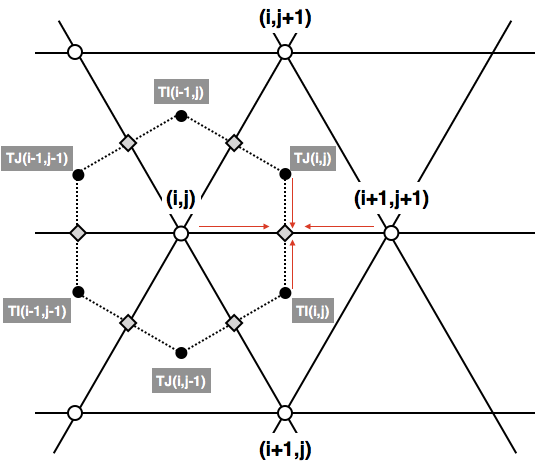
\includegraphics[scale=.4]{figs/diffusion_diff.png}
 \caption{Interpolation for \src{dscl}}\label{f:interpolation_for_dscl}
\end{figure}


The last part of this subroutine is as follows.


\begin{LstF90}[name=diffusion,firstnumber=last]
  if ( ADM_have_pl ) then
     n = ADM_gslf_pl

     do l = 1, ADM_lall_pl
     do k = 1, ADM_kall

        do d = 1, ADM_nxyz
           do v = ADM_gmin_pl, ADM_gmax_pl
              ij   = v
              ijp1 = v + 1
              if( ijp1 == ADM_gmax_pl+1 ) ijp1 = ADM_gmin_pl

              vt_pl(ij,d) = ( ( + 2.0_RP * coef_intp_pl(v,1,d,l) &
                                - 1.0_RP * coef_intp_pl(v,2,d,l) &
                                - 1.0_RP * coef_intp_pl(v,3,d,l) ) * scl_pl(n   ,k,l) &
                            + ( - 1.0_RP * coef_intp_pl(v,1,d,l) &
                                + 2.0_RP * coef_intp_pl(v,2,d,l) &
                                - 1.0_RP * coef_intp_pl(v,3,d,l) ) * scl_pl(ij  ,k,l) &
                            + ( - 1.0_RP * coef_intp_pl(v,1,d,l) &
                                - 1.0_RP * coef_intp_pl(v,2,d,l) &
                                + 2.0_RP * coef_intp_pl(v,3,d,l) ) * scl_pl(ijp1,k,l) &
                            ) / 3.0_RP
           enddo
        enddo

        dscl_pl(:,k,l) = 0.0_RP

        do v = ADM_gmin_pl, ADM_gmax_pl
           ij   = v
           ijm1 = v - 1
           if( ijm1 == ADM_gmin_pl-1 ) ijm1 = ADM_gmax_pl ! cyclic condition

           dscl_pl(n,k,l) = dscl_pl(n,k,l) &
                          + ( coef_diff_pl(v-1,XDIR,l) * ( vt_pl(ijm1,XDIR) + vt_pl(ij,XDIR) ) &
                            + coef_diff_pl(v-1,YDIR,l) * ( vt_pl(ijm1,YDIR) + vt_pl(ij,YDIR) ) &
                            + coef_diff_pl(v-1,ZDIR,l) * ( vt_pl(ijm1,ZDIR) + vt_pl(ij,ZDIR) ) &
                            ) * 0.5_RP * ( kh_pl(n,k,l) + kh_pl(ij,k,l) )
        enddo

     enddo
     enddo
  else
     dscl_pl(:,:,:) = 0.0_RP
  endif

  call DEBUG_rapend('OPRT_diffusion')

  return
end subroutine OPRT_diffusion
\end{LstF90}

The last part is for calculation for the pole region.
Variable \src{ADM_have_pl} is \src{.true.} if this process manages pole
region in original \NICAM.
For the kernel program, also set as \src{.true.} in \file{problem_size.inc}.



\subsection{Input data and result}

Max/min/sum of input/output data of the kernel subroutine are output as
a log.
%
Below is an example of \src{$IAB_SYS=Ubuntu-gnu-ompi} case.


\begin{LstLog}
 ### Input ###
 +check[check_dscl      ] max=  6.1941315670898286E-08,min= -7.0374144752795210E-08,sum= -2.7407850230958588E-07
 +check[check_dscl_pl   ] max=  2.2139244811324830E-08,min= -6.0170678327656930E-11,sum=  1.8274579608905828E-07
 +check[scl             ] max=  1.6578626530298903E-11,min= -1.2670212860993856E-11,sum= -2.0289014286353776E-10
 +check[scl_pl          ] max=  1.9358849576453664E-11,min= -8.2853331106472899E-12,sum=  1.1445754720677440E-09
 +check[kh              ] max=  2.8341305529772246E+12,min=  6.7659597088284981E+10,sum=  6.0439053980501018E+17
 +check[kh_pl           ] max=  2.8334094314435532E+12,min=  6.7659597088284981E+10,sum=  4.3486317454839525E+14
 ### Output ###
 +check[dscl            ] max=  6.1941315670898286E-08,min= -7.0374144752795210E-08,sum= -2.7407850230958588E-07
 +check[dscl_pl         ] max=  2.2139244811324830E-08,min= -6.0170678327656930E-11,sum=  1.8274579608905828E-07
 ### Validation : grid-by-grid diff ###
 +check[check_dscl      ] max=  0.0000000000000000E+00,min=  0.0000000000000000E+00,sum=  0.0000000000000000E+00
 +check[check_dscl_pl   ] max=  0.0000000000000000E+00,min=  0.0000000000000000E+00,sum=  0.0000000000000000E+00
 *** Finish kernel
\end{LstLog}

Check the lines below \src{``Validation : grid-by-grid diff''} line,
that shows difference between calculated output array and
pre-calculated reference array.
These should be zero or enough small to be acceptable.

There are sample output log files in \file{reference/}
in each kernel program directory, for reference purpose.


\subsection{Sample of perfomance result}

Here's an example of the performance result part of the log output.
Below is an example executed with the machine environment described in \autoref{s:measuring_env}.
%
Note that in this program kernel part is iterated one time.

\begin{LstLog}
 *** Computational Time Report
 *** ID=001 : MAIN_dyn_diffusion               T=     0.028 N=      1
 *** ID=002 : OPRT_diffusion                   T=     0.028 N=      1
\end{LstLog}

